\documentclass[../practica_01.tex]{subfiles}

\begin{document}

    \begin{enumerate}
        \item $x^2+y^2+z^2-6x+4y-2z = 11$

            $P_0 = (a,b,c) \wedge b: (x-a)^2+(y-b)^2+(z-c)^2 = r^2$ entonces

            b es un circulo con centro en $P_0$ y radio $r$

            $x^2 + y^2 + z^2 - 2ax + a^2 - 2by + b^2 - 2cz + c^2 = x^2 + y^2 + z^2 - 6x + 4y - 2z + j = 11 + j$

            \begin{itemize}
                \item $-2ax = -6x \equiv a = 3$
                \item $-2by = 4y \equiv b = -2$
                \item $-2cz = -2z \equiv c = 1$
            \end{itemize}

            $(x-3)^2+(y+2)^2+(z-1)^2 \equiv$
            
            $(x^2 - 6x + 9) + (y^2 + 4y + 4) + (z^2 - 2z + 1) = 11 + j \equiv$
            
            $(x^2 + y^2 + z^2) - 6x + 4y - 2z + 9 + 4 + 1 = 11 + j \equiv$

            $(x^2 + y^2 + z^2) - 6x + 4y - 2z + 14 = 11 + j \equiv $

            $(x^2 + y^2 + z^2) - 6x + 4y - 2z = 25$
            
            Es un circulo con centro en $(3,-2,1)$ y radio $5$

            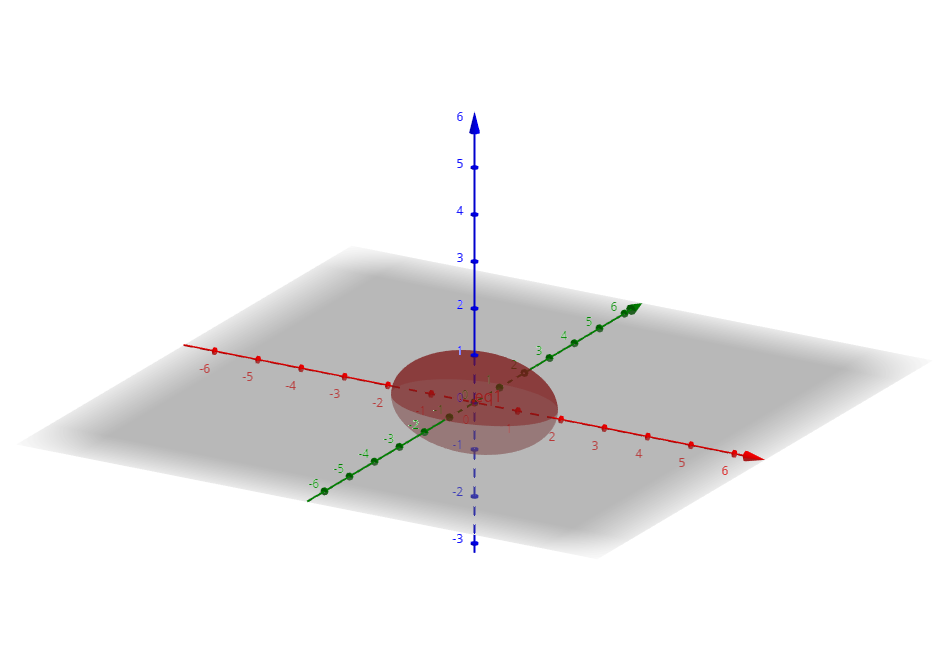
\includegraphics[scale=0.2]{ej02/resources/2a.png} $ $

        \item $4x^2 + 4y^2 + 4z^2 - 8x + 16y = 1$

            $4(x^2 + y^2 + z^2 - 2x + 4y) = 1 \equiv$

            $x^2 + y^2 + z^2 - 2x + 4y = \frac{1}{4}$

            $x^2 + y^2 + z^2 - 2ax + a^2 - 2by + b^2 - 2cz + c^2 = x^2 + y^2 + z^2 - 2x + 4y = \frac{1}{4}$

            $x^2 + y^2 + z^2 - 2ax + a^2 - 2by + b^2 - 2cz + c^2 = x^2 + y^2 + z^2 - 2x + 4y = \frac{1}{4}$

            \begin{itemize}
                \item $-2ax = -2x \equiv a = 1$
                \item $-2by = 4y \equiv b = -2$
                \item $-2cz = 0 \equiv c = 0$
            \end{itemize}

            $(x-1)^2+(y+2)^2+(z)^2 \equiv$

            $x^2 + -2x + 1 + y^2 + 4y + 4 + z^2 \equiv$

            $(x^2 + y^2 + z^2 - 2x + 4y) + 5 = \frac{1}{4} + 5 \equiv$

            $x^2 + y^2 + z^2 - 2x + 4y + 5 = \frac{21}{4} $

            $(x-1)^2+(y+2)^2+(z)^2 = \frac{21}{4} $

            Es un circulo con centro en $(1,-2,0)$ y radio $\frac{\sqrt{21}}{2}$

            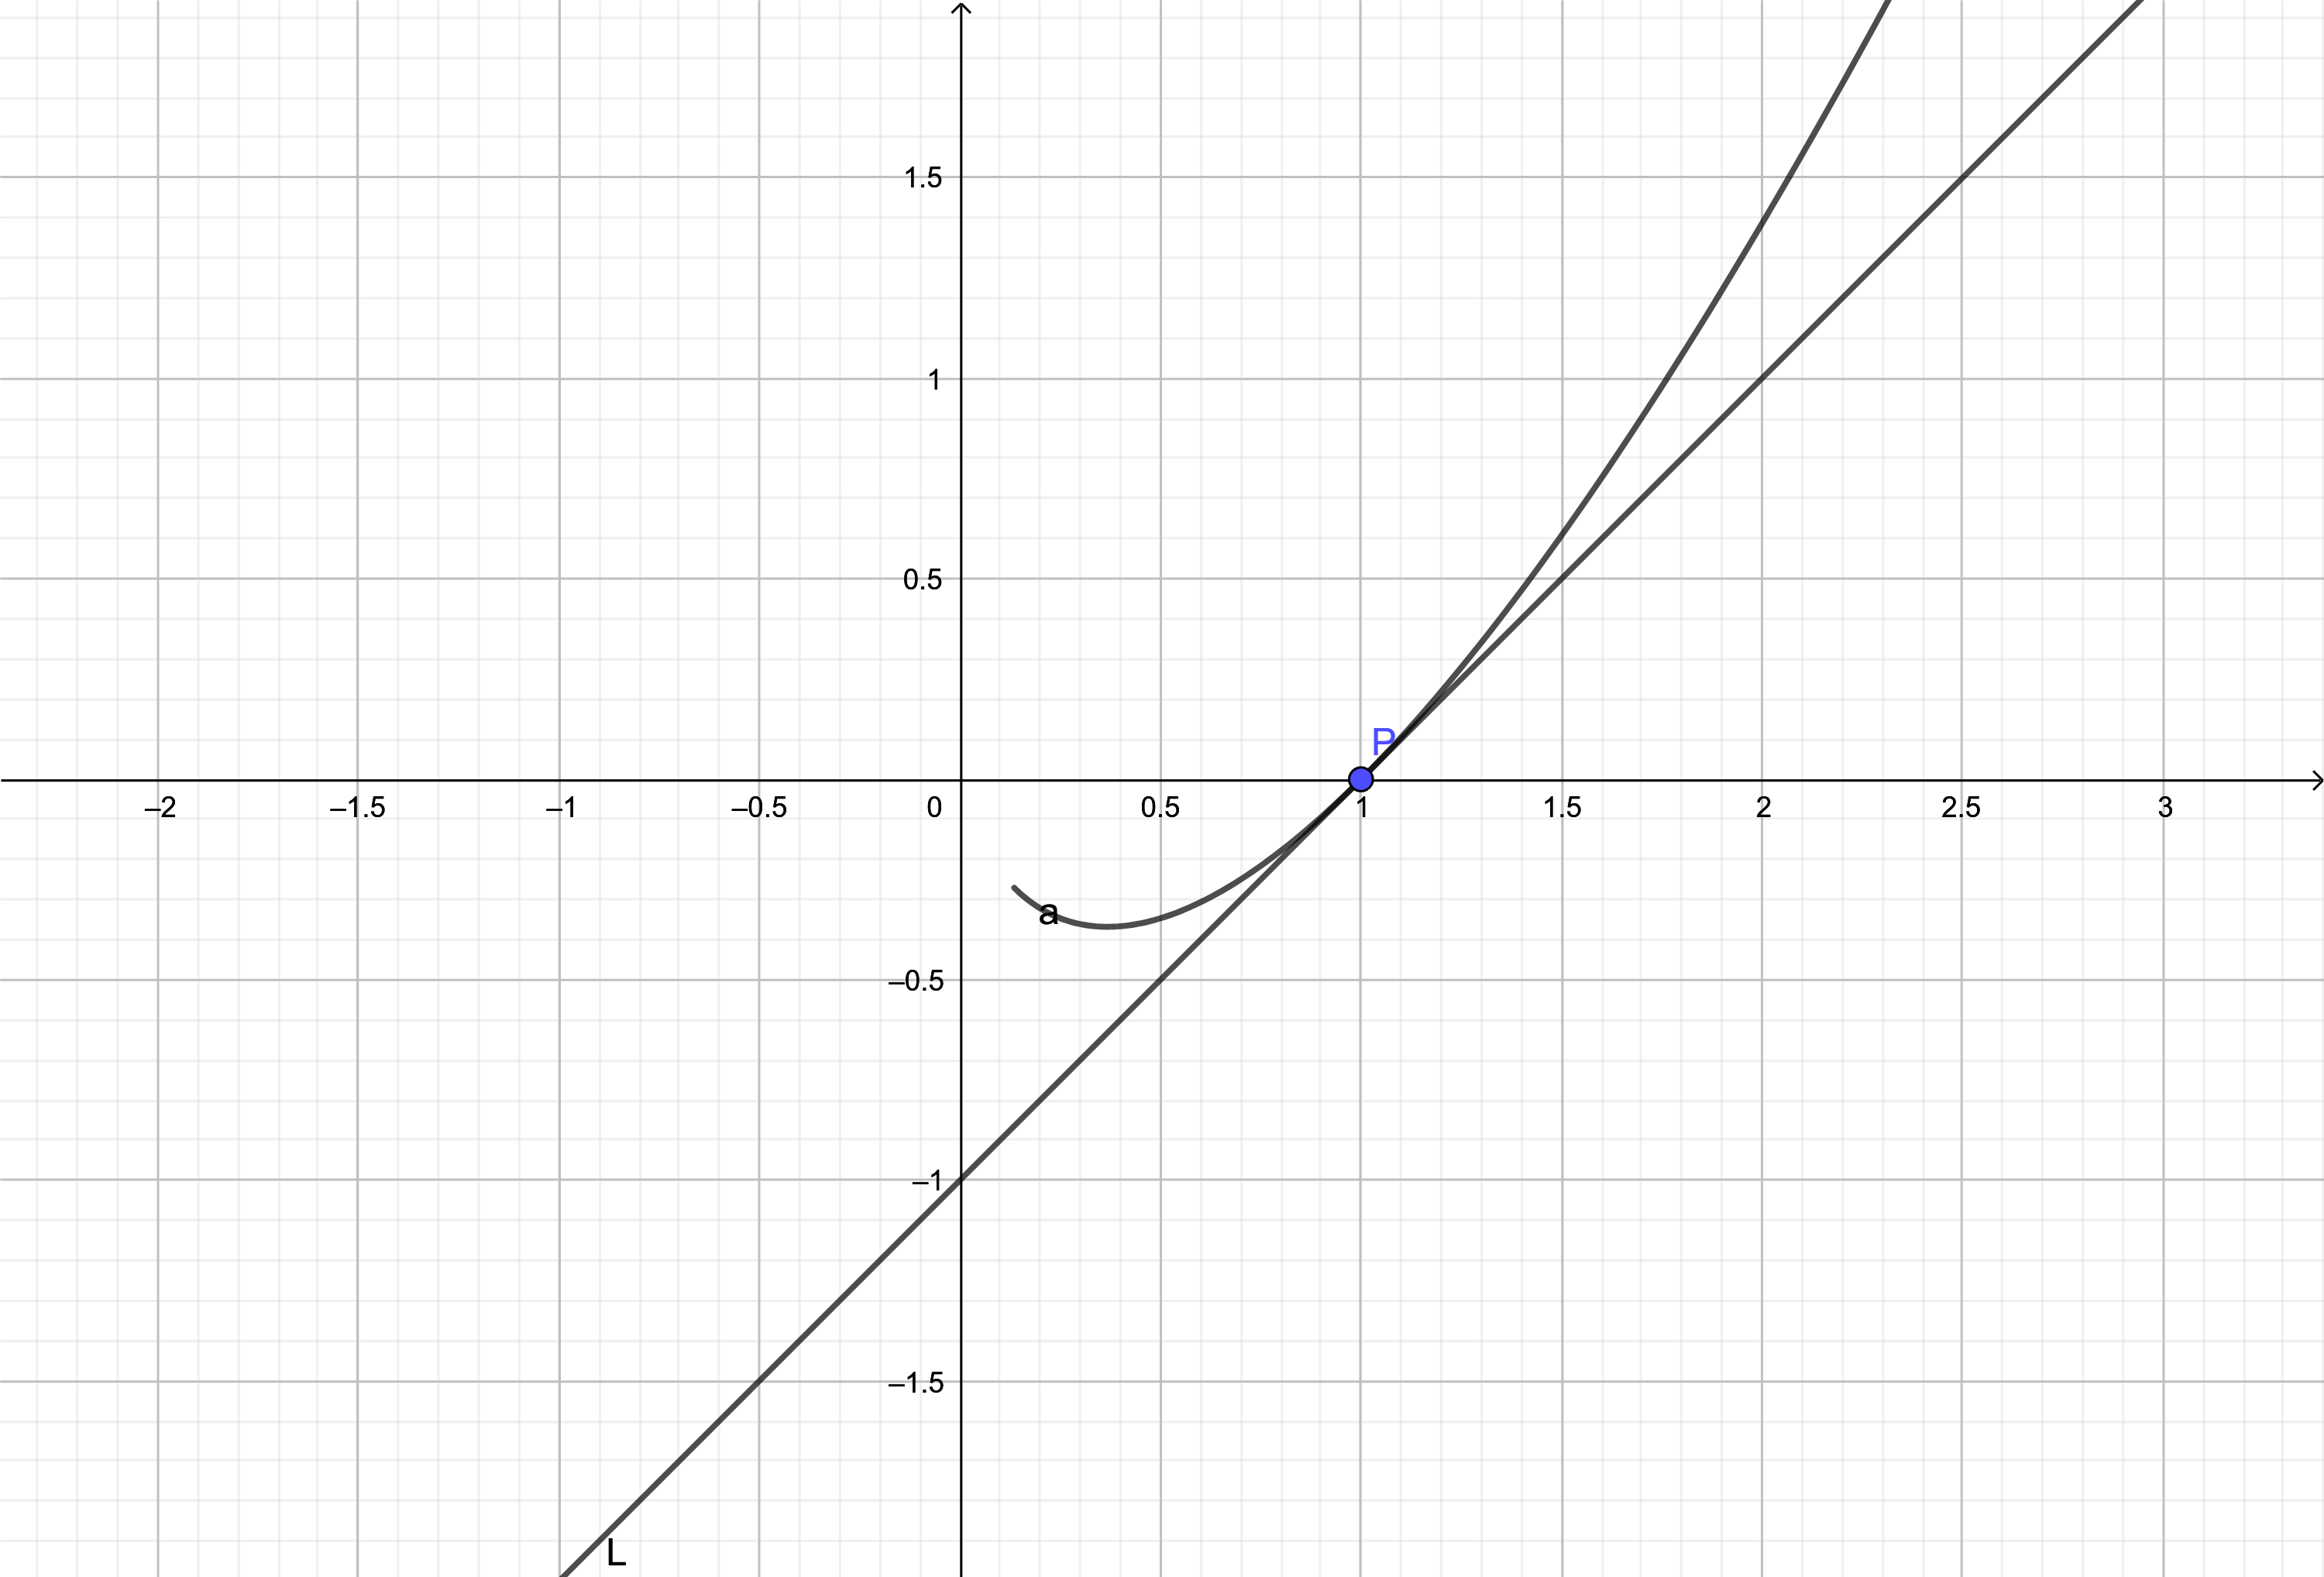
\includegraphics[scale=0.2]{ej02/resources/2b.png} $ $

    \end{enumerate}

\end{document}